\chapter{Concepts}

\section{Antifragile Attributes}
\label{sec:antifragileattributes}
\begin{table}[!h]
	\begin{center}
		\resizebox{\textwidth}{!}{%
		\begin{tabular}{@{}llll@{}}
			\toprule
			\textbf{Attribute} & \textbf{Variety} & \textbf{Behaviour} & \textbf{Sources} \\ \midrule
			Top Down C\&C & \Gls{attenuatevariety} & Engineering Resilience & \parencite{Botjes2020} \\
			Micro-Management & \Gls{attenuatevariety} & Engineering Resilience & \parencite{Botjes2020} \\
			Redundancy & \Gls{attenuatevariety} & Systems Resilience & \parencite{Botjes2020} \\
			Modularity & \Gls{attenuatevariety} & Systems Resilience & \parencite{Botjes2020} \\
			Loosely coupled & \Gls{attenuatevariety} & Systems Resilience & \parencite{Botjes2020} \\
			Diversity & \Gls{amplifyvariety} & \acrshort{cas} Resilience & \parencite{Botjes2020} \\
			Optionality & \Gls{amplifyvariety} & \acrshort{cas} Resilience & \parencite{Taleb2012} \\
			Non-Monotonicity & \Gls{amplifyvariety} & \acrshort{cas} Resilience & \parencite{Botjes2020} \\
			Emergence & \Gls{amplifyvariety} & \acrshort{cas} Resilience & \parencite{Botjes2020} \\
			Self-Organisation & \Gls{amplifyvariety} & \acrshort{cas} Resilience & \parencite{Botjes2020} \\
			Insert low-level stress & \Gls{amplifyvariety} & \acrshort{cas} Resilience & \parencite{Botjes2020} \\
			Network-connections & \Gls{amplifyvariety} & \acrshort{cas} Resilience & \parencite{Botjes2020} \\
			Fail Fast & \Gls{amplifyvariety} & \acrshort{cas} Resilience & \parencite{Botjes2020} \\
			\Gls{resourcestoinvest} & \Gls{amplifyvariety} & Antifragile & \parencite{Botjes2020,Taleb2012} \\
			\Gls{senecabarbell} & \Gls{amplifyvariety} & Antifragile & \parencite{Taleb2012,Botjes2020} \\
			\Gls{insertrandomness} & \Gls{amplifyvariety} & Antifragile & \parencite{Taleb2012,Botjes2020} \\			
			\Gls{reducenaiveintervention} & \Gls{amplifyvariety} & Antifragile & \parencite{Taleb2012,Botjes2020} \\
			\Gls{skininthegame} & \Gls{amplifyvariety} & Antifragile & \parencite{Taleb2012,Botjes2020} \\
			\Gls{personalmastery} & \Gls{attenuatevariety} \& \Gls{amplifyvariety} & Learning Organisation & \parencite{Botjes2020} \\
			\Gls{sharedmentalmodels} & \Gls{attenuatevariety} \& \Gls{amplifyvariety} & Learning Organisation & \parencite{Botjes2020} \\
			\Gls{buildingsharedvision} & \Gls{attenuatevariety} \& \Gls{amplifyvariety} & Learning Organisation & \parencite{Botjes2020} \\
			\Gls{teamlearning} & \Gls{attenuatevariety} \& \Gls{amplifyvariety} & Learning Organisation & \parencite{Botjes2020} \\
			\Gls{systemsthinking} & \Gls{attenuatevariety} \& \Gls{amplifyvariety} & Learning Organisation & \parencite{Botjes2020} \\
			\bottomrule
		\end{tabular}
		}
		\caption{Concepts of Antifragile}
	\end{center}
\end{table}

While \parencite[p. 66]{Botjes2020} defined optionality as part of diversity the definitions are slightly different. In the case of this research it is applicable to use both the concepts.
\begin{remark}
Needs some references to taleb and others to do so in the case of my research.
\end{remark}

\section{Questions for Interviews}
\label{sec:questionsforinterviews}
The questions for the interviews are limited by the constraint of time of an interview. Because of this time constraint I limited the number of questions to five. However the five questions do cover the attributes of \gls{antifragile} and the concept of \gls{ea}.


\subsection{Interview Question 1}

\subsection{Interview Question 2}

\subsection{Interview Question 3}

\subsection{Interview Question 4}

\subsection{Interview Question 5}


Architects use an \gls{archframework} for describing \acrshort{ea}. Most of the frameworks use a layered approach for specific viewpoints on a system. The most used layers are business, information, applications, and technology. \textcite[p. 189]{Ylimaeki2005} suggests that \acrshort{ea} is an approach for controlling the complexity and constant changes in the business environment of an organisation, enabling alignment between the business vision, business requirements and information systems.


Most people answer that the opposite of \gls{fragile} is \gls{robust}, \gls{resilient}, solid, or something of the sort. However, the \gls{resilient}, \gls{robust} (and company) are items that neither break nor improve, so you would not need to write anything on them — have you ever seen a package with \gls{robust} in thick green letters stamped on it? Logically, the exact opposite of a \gls{fragile} parcel would be a package on which one has written; please mishandle or please handle carelessly. Its contents would not just be unbreakable but would benefit from shocks and a wide array of trauma \parencite{Taleb2012}. \textcite[p. 32]{Botjes2020} mentions that almost all if not all papers on antifragility and resilience use the term stressor for an event from outside the system that causes stress.



\textcite[p. 32]{Botjes2020} mentions that almost all if not all papers on antifragility and resilience use the term stressor for an event from outside the system that causes stress. 

\begin{figure}[h!]
	\centering
	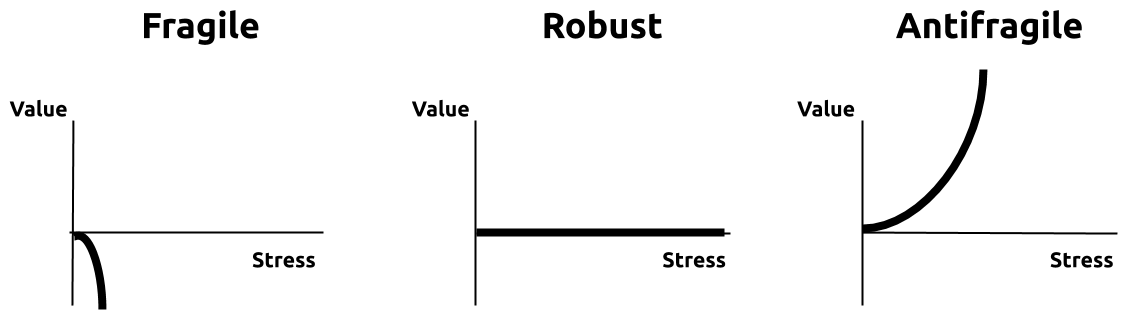
\includegraphics[width=0.7\linewidth]{images/eaal-triad}
	\caption[EAAL Triad]{\acrfull{eaal} Triad \parencite{Botjes2020}}
	\label{fig:eaal-triad}
\end{figure}